%% orthologue_prediction.tex
%% Author: Leighton Pritchard
%% Copyright: James Hutton Institute
%% A brief introduction to orthologues, and their prediction

% SUBSECTION: Why orthologues?
\subsection{What's so important about orthologues?}

% Why focus on orthologues
\begin{frame}
  \frametitle{Why focus on orthologues?}
  Formalise the idea of \textit{corresponding genes} in different organisms. \\
  Orthologues serve two purposes:
  \begin{itemize}
    \item \textbf{Evolutionary equivalence}
    \item \textbf{Functional equivalence} (``The Ortholog Conjecture''\footnote{\tiny{Chen and Zhang (2012) \textit{PLoS Comp. Biol.} \textbf{8}:e1002784 \href{http://dx.doi.org/10.1371/journal.pcbi.1002784}{doi:10.1371/journal.pcbi.1002784}}})
  \end{itemize}
  Applications in comparative genomics, functional genomics and phylogenetics.\footnote{\tiny{Dessimoz (2011) \textit{Brief. Bioinf.} \textbf{12}:375-376 \href{http://dx.doi.org/10.1093/bib/bbr057}{doi:10.1093/bib/bbr057}}} \\
  Over 30 databases attempt to describe orthologous relationships (\href{http://questfororthologs.org/orthology_databases
}{http://questfororthologs.org/orthology\_databases}\footnote{\tiny{Altenhoff and Dessimoz (2009) \textit{PLoS Comp. Biol.} \textbf{5}:e1000262 \href{http://dx.doi.org/10.1371/journal.pcbi.1000262}{doi:10.1371/journal.pcbi.1000262}}})
\end{frame}

% Orthologue-finding methods
\begin{frame}
  \frametitle{Finding orthologues}
      Multiple methods and databases%
\footnote{\tiny{Kristensen \textit{et al}. (2011) \textit{Brief. Bioinf.} \textbf{12}:379-391 \href{http://dx.doi.org/10.1093/bib/bbr030}{doi:10.1093/bib/bbr030}}}$^,$%
\footnote{\tiny{Trachana \textit{et al}. (2011) \textit{Bioessays} \textbf{33}:769-780 \href{http://dx.doi.org/10.1002/bies.201100062}{doi:10.1002/bies.201100062}}}$^,$%
\footnote{\tiny{Salichos and Rokas (2011) \textit{PLoS One} \textbf{6}:e18755 \href{http://dx.doi.org/10.1371/journal.pone.0018755.g006}{doi:10.1371/journal.pone.0018755.g006}}}
  \begin{columns}[T]    \begin{column}{6cm}
      \begin{itemize}
        \item \textbf{Pairwise genome}
        \begin{itemize}
          \item \href{http://armchairbiology.blogspot.co.uk/2012/07/on-reciprocal-best-blast-hits.html}{RBBH} (aka BBH, RBH), \href{http://link.springer.com/protocol/10.1007/978-1-59745-515-2_7}{RSD}, \href{http://inparanoid.sbc.su.se/cgi-bin/index.cgi}{InParanoid}, \href{http://roundup.hms.harvard.edu/}{RoundUp}
        \end{itemize}
        \item \textbf{Multi-genome}
        \begin{itemize}
          \item Graph-based: \href{http://www.ncbi.nlm.nih.gov/COG/}{COG}, \href{http://eggnog.embl.de/}{eggNOG}, \href{http://cegg.unige.ch/orthodb7}{OrthoDB}, \href{http://orthomcl.org/orthomcl/}{OrthoMCL}, \href{http://omabrowser.org/cgi-bin/gateway.pl}{OMA}, \href{http://multiparanoid.sbc.su.se/}{MultiParanoid}
          \item Tree-based: \href{http://www.treefam.org/}{TreeFam}, \href{http://www.ensembl.org/info/genome/compara/index.html}{Ensembl Compara}, \href{http://phylomedb.org/}{PhylomeDB}, \href{https://trac.nbic.nl/loft/}{LOFT}
        \end{itemize}
      \end{itemize}
    \end{column}
    \begin{column}{4cm}
      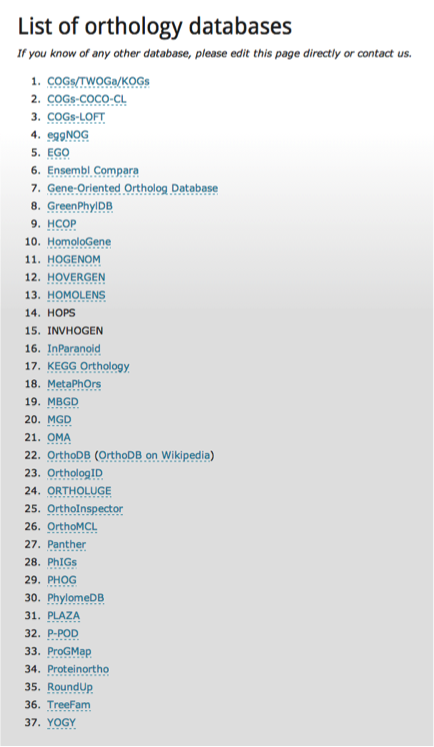
\includegraphics[height=0.6\textheight]{images/orthology_databases}      
    \end{column}
  \end{columns}
\end{frame}

